\section{Localização dos Usuários}

O Sistema TRUE obtém a localização dos usuários no ambiente por meio de coordenadas dos mesmos em relação ao \textit{Kinect}. Para saber o quanto essas coordenadas são confiáveis foram realizados alguns testes que resultaram em gráficos que comparam as coordenadas obtidas pelo sistema e as coordenadas reais.

As coordenadas $\displaystyle (x, y, z)$ obtidas pelo sistema são coordenas de um plano cartesiano de três dimensões em que o ponto $\displaystyle (0, 0, 0)$ corresponde a posição do \textit{Kinect}. Os valores das coordenadas que realmente são utilizadas para estimar a localização do usuário no ambiente são os valores nos eixos $\displaystyle x$ e $\displaystyle z$. Os valores do eixo $\displaystyle y$ correspondem somente a altura do centro de massa geométrico do usuário rastreado. Portanto, os testes desenvolvidos aferiram somente os valores obtidos pelo Sistema TRUE nos eixos $\displaystyle x$ e $\displaystyle z$.

\subsection{Teste dos valores no eixo $\displaystyle z$}

	Os valores obtidos no eixo $\displaystyle z$ correspondem aos valores de profundidade do usuário rastreado em relação ao \textit{Kinect}. Portanto, para testar a precisão do Sistema TRUE foi realizado o seguinte teste: um objeto (uma caixa de papelão) foi colocada em frente ao sensor, como mostrado na Figura~\ref{fig:teste-z}, em diferentes distâncias do mesmo (1 metro, 2 metros, 3 metros, 4 metros, 4,057 metros). Para cada distância, foram anotados alguns valores obtidos pelo sistema, mostrados na Tabela~\ref{tab:valores-z}, e foram obtidas diferentes imagens do Sistema TRUE mostradas na Figura~\ref{fig:distancias}. Então esses valores foram inseridos em um gráfico e comparado com os valores reais.

	\begin{figure}[htb]
		\begin{center}
			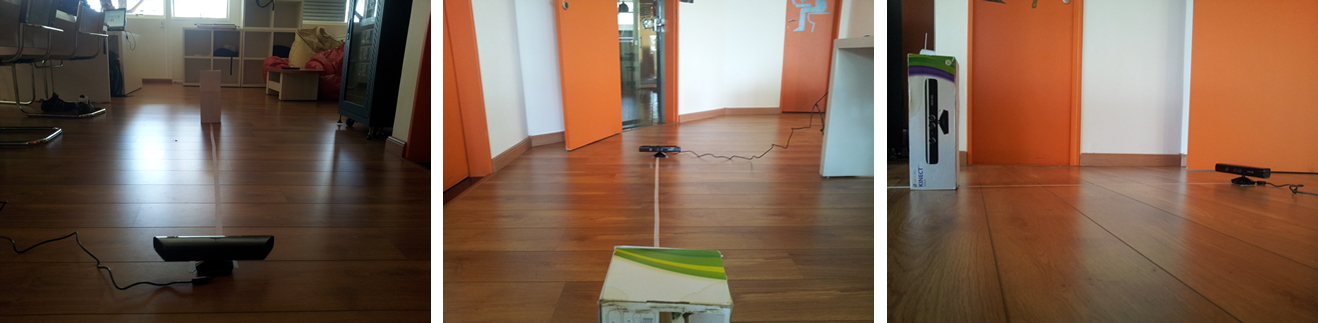
\includegraphics[scale=0.35]{figuras/5.Testes/teste-eixoz.png}
		\end{center}
		\caption{Fotos retiradas no teste realizado para aferir os valores obtidos no eixo $\displaystyle z$.}
		\label{fig:teste-z}
	\end{figure}

	\begin{figure}[htb]
		\begin{center}
			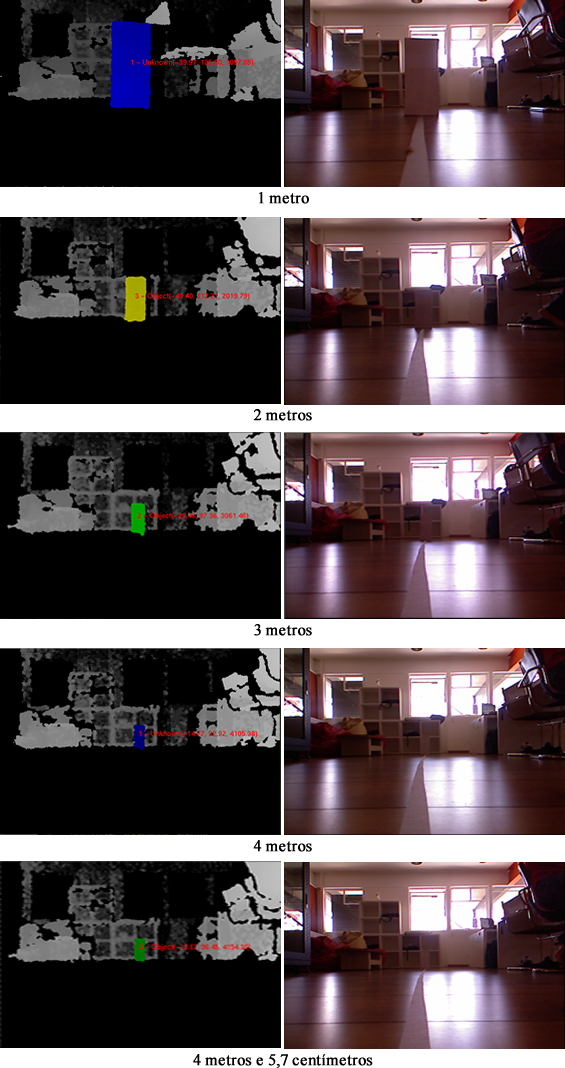
\includegraphics[scale=0.6]{figuras/5.Testes/eixoz-imgs.png}
		\end{center}
		\caption{Fotos obtidas pelo Sistema TRUE no teste realizado para os valores do eixo $\displaystyle z$.}
		\label{fig:distancias}
	\end{figure}

		\begin{table}[h]
		\begin{center}
			\caption{Valores obtidos pelo Sistema TRUE.}
			\begin{tabular}{|c|c|c|c|c|}
				\hline \bf Distância do objeto ao \textit{Kinect} (mm) & \multicolumn{4}{|c|}{\bf Valores obtido pelo Sistema TRUE (mm)} \\
				\hline
				\hline 1000,00 & 1007,56 & 1006,64 & 1003,21 & 1007,56 \\
				\hline 2000,00 & 2020,27 & 2021,17 & 2020,55 & 2020,48 \\
				\hline 3000,00 & 3058,70 & 3057,60 & 3062,01 & 3059,10 \\
				\hline 4000,00 & 4115,31 & 4110,25 & 4111,59 & 4114,80 \\
				\hline 4057,00 & 4166,35 & 4163,83 & 4166,45 & 4168,75 \\
				\hline
			\end{tabular}
		\end{center}
		\label{tab:valores-z}
	\end{table}

	Os valores obtidos no teste foram inseridos em um gráfico representado pela Figura~\ref{fig:grafico-z}. Neste gráfico existem duas retas: uma reta preta que representa valores ideias que batem com os valores reais; e uma reta vermelha que representa os valores obtidos pelo sistema. Como observado, a medida que o objeto se afasta do \textit{Kinect} as diferenças entre os valores reais e os valores obtidos aumetam. Contudo, essa diferença é de poucos centímetros.

	\begin{figure}[htb]
		\begin{center}
			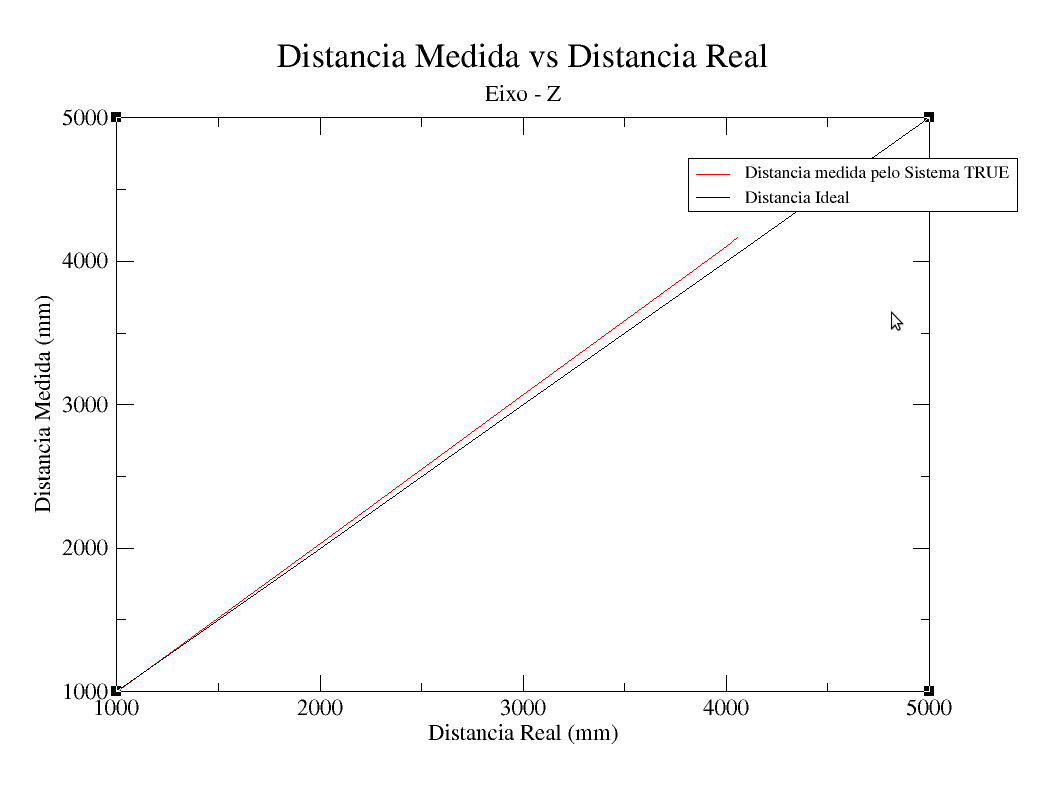
\includegraphics[scale=0.4]{figuras/5.Testes/grafico-eixo-z.png}
		\end{center}
		\caption{Gráfico comparativo entre os valores obtidos pelo Sistema TRUE e os valores reais.}
		\label{fig:grafico-z}
	\end{figure}

	Pelos resultados deste teste, pode-se concluir que o Sistema TRUE fornece informações sobre localização dos usuários bem precisas e confiáveis podendo ter erros de poucos centímetros que não prejudicam a integridade das informações. 

	Através deste teste, também foi possível obter a distância máxima e mínima que o usuário deve estar do \textit{Kinect} para que o sistema consiga rastrear-lo e estimar sua localização. A distância mínima é de $\displaystyle 48,3 cm$ e a máxima de $\displaystyle 4,057 m$.

\subsection{Teste dos valores no eixo $\displaystyle x$}

	Os valores obtidos no eixo $\displaystyle x$ mostram o quanto o usuário rastreado está a direita ou a esquerda em relação ao \textit{Kinect}. Portanto, para testar a precisão do Sistema TRUE foi realizado o seguinte teste: um objeto (uma caixa de papelão) foi colocada a uma distância fixa de 3 metros do sensor e colocada em diferentes posições ao longo do eixo $\displaystyle x$ (0, $\displaystyle \pm33 cm$, $\displaystyle \pm66 cm$, $\displaystyle \pm99 cm$), como mostrado na Figura~\ref{fig:teste-eixox}. Para cada posição, alguns valores obtidos pelo Sistema TRUE foram anotados, mostrados na Tabela~\ref{tab:valores-x}, e algumas imagens do sistema foram obtidas, mostradas na Figura~\ref{fig:eixox-imgs}. Então esses valores foram inseridos em um gráfico e comparados com os valores reais.

	\begin{figure}[htb]
		\begin{center}
			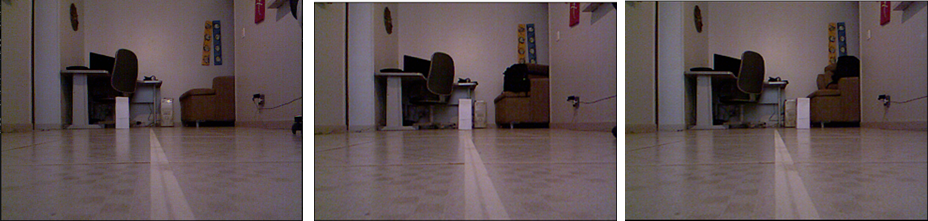
\includegraphics[scale=0.45]{figuras/5.Testes/teste-eixox.png}
		\end{center}
		\caption{Fotos retiradas no teste realizado para aferir os valores obtidos no eixo $\displaystyle x$.}
		\label{fig:teste-eixox}
	\end{figure}

	\begin{figure}[htb]
		\begin{center}
			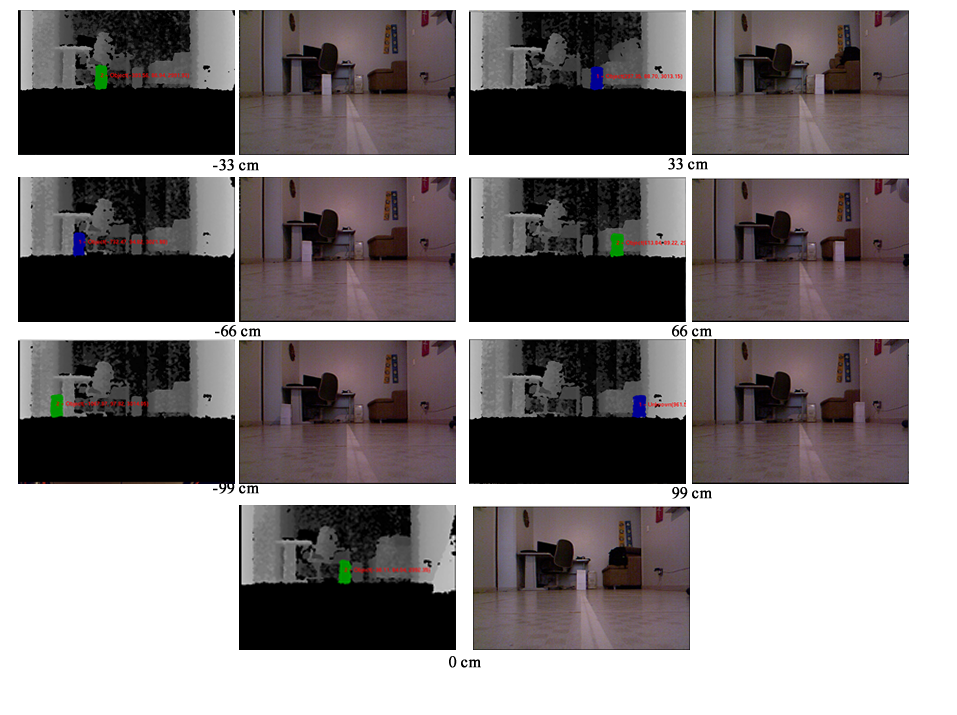
\includegraphics[scale=0.55]{figuras/5.Testes/eixox-imgs.png}
		\end{center}
		\caption{Fotos obtidas pelo Sistema TRUE no teste realizado para os valores do eixo $\displaystyle x$.}
		\label{fig:eixox-imgs}
	\end{figure}

	\begin{table}[h]
		\begin{center}
			\caption{Valores obtidos pelo Sistema TRUE.}
			\begin{tabular}{|c|c|c|c|c|}
				\hline \bf Posição do objeto & \multicolumn{4}{|c|}{\bf Valores obtido}\\
							 \bf ao longo do eixo $\displaystyle x$ (mm) & \multicolumn{4}{|c|}{\bf pelo Sistema TRUE (mm)}\\
				\hline
				\hline 0    & -31,82   & -34,5    & -31,39   & -33,51 \\
				\hline 0    & -35,40   & -33,38   & -35,03   & -31,33  \\
				\hline 330  & 296,94   & 298,16   & 298,95   & 296,21 \\
				\hline -330 & -387,42  & -391,42  & -392,54  & -389,96 \\
				\hline 660  & 615,53   & 615,93   & 614,71   & 614,22 \\
				\hline -660 & -727,04  & -733,95  & -731,34  & -732,18 \\
				\hline 990  & 963,85   & 962,64   & 961,80   & 962,95 \\
				\hline -990 & -1069,32 & -1068,00 & -1070,48 & -1069,35 \\
				\hline
			\end{tabular}
		\end{center}
		\label{tab:valores-x}
	\end{table}

	Os valores obtidos no teste foram inseridos em um gráfico representado pela Figura~\ref{fig:grafico-eixox}. Neste gráfico existem duas retas: uma reta preta que representa os valores reais; e uma reta vermelha que representa os valores obtidos pelo sistema. Como observado, existe uma diferença constante de poucos centímetros ao longo de toda a reta, ou seja, com o objeto fixo a uma ditância de 3 metros do \textit{Kinect}, o Sistema TRUE consegue fazer estimativas das coordenadas no $\displaystyle x$ com erro de poucos centímetros. Um erro pequeno que não prejudica a integridade dos valores obtidos pelo sistema.

	\begin{figure}[htb]
		\begin{center}
			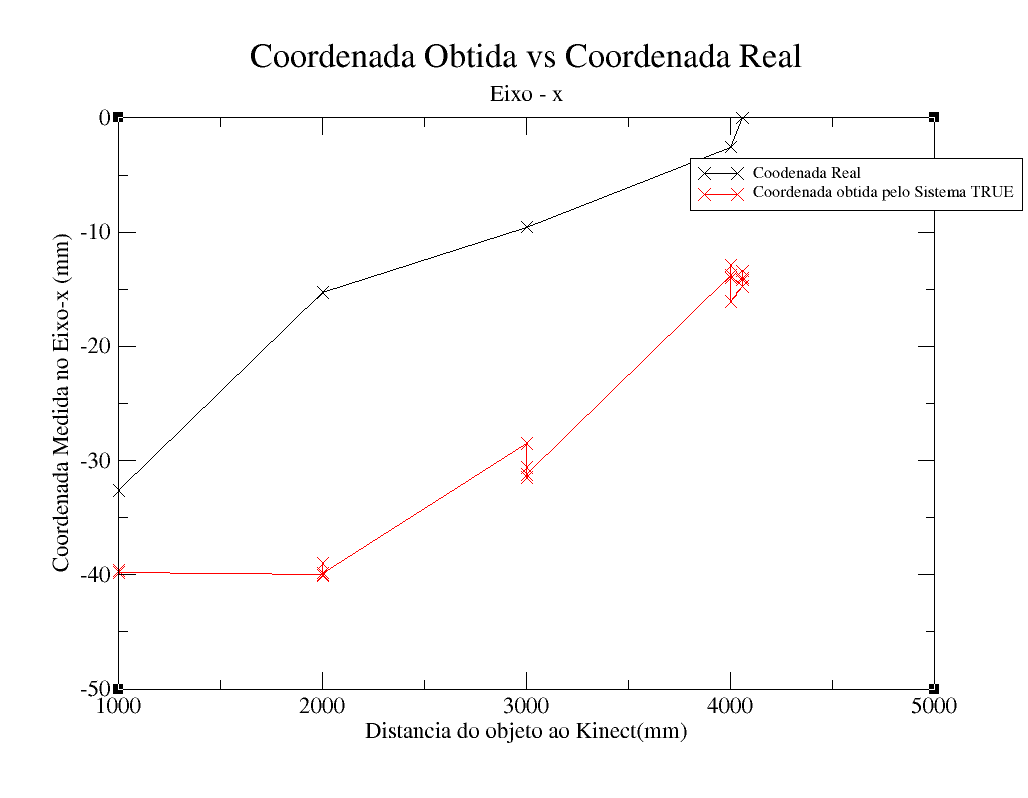
\includegraphics[scale=0.4]{figuras/5.Testes/grafico-eixo-x.png}
		\end{center}
		\caption{Gráfico comparativo entre os valores obtidos pelo Sistema TRUE e os valores reais.}
		\label{fig:grafico-eixox}
	\end{figure}

































